\documentclass[conference]{IEEEtran}
\IEEEoverridecommandlockouts
\usepackage{cite}
\usepackage{amsmath,amssymb,amsfonts}
\usepackage{algorithmic}
\usepackage{graphicx}
\usepackage{textcomp}
\usepackage{xcolor}
\def\BibTeX{{\rm B\kern-.05em{\sc i\kern-.025em b}\kern-.08em
		T\kern-.1667em\lower.7ex\hbox{E}\kern-.125emX}}
\begin{document}
	
	\title{Integration of 75MW Solar PV Plant: Transmission System Design Analysis}
	
	\author{\IEEEauthorblockN{Brent Dickinson}
		\IEEEauthorblockN{Tianci}
	}
	
	\maketitle
	
\begin{abstract}
	This report presents the design and analysis of transmission system modifications required to integrate a new 75MW solar PV plant while addressing existing system reliability concerns. The study evaluates various transmission line and transformer options to determine the most cost-effective solution that maintains system stability under both normal and N-1 contingency conditions.
\end{abstract}

\section{Introduction}
The integration of renewable energy sources into existing power grids presents technical challenges. We analyze the design requirements and potential solutions for integrating a new 75 MW utility-scale solar photo-voltaic (PV) facility into an existing 37-bus power system while also solving current reliability issues.

We aim to find the most cost-effective transmission system additions required to integrate 75 MW of solar generation at the NEWSOLAR substation. That goal is subordinate to the constraints of ensuring system reliability through dual transmission paths to the facility and resolving existing system violations identified using PowerWorld's contingency analysis.

The design must satisfy the following constraints. Bus voltages must be maintained between 0.95 and 1.10 per unit, while keeping all line flows below 100\% of their thermal limits. The system must maintain stability under both normal operation and N-1 contingency conditions. Additionally, redundant transmission paths to the NEWSOLAR substation are required. The system must accommodate the solar plant operating at both full capacity (75 MW) and offline conditions.

Our approach incorporates contingency analysis, evaluation of available transmission corridors and voltage levels, and assessment of various conductor types and their associated costs. We consider transformer options and substation modifications. We conduct an economic analysis incorporating both capital costs and five-year loss reduction benefits.

Initial contingency analysis reveals specific reliability concerns in the OAK69-BUCKEYE69-APPLE69 corridor, which must be addressed alongside the integration of the new solar facility. The following sections detail the technical analysis, proposed solutions, and economic justification for the recommended design.

\section{Initial System Analysis}
\subsection{Base Case Evaluation}
The existing 37-bus system operates with a total load of 826.3 MW and 275.5 Mvar, served by ten generators producing 837.7 MW. System losses are approximately 10.7 MW, representing 1.3\% of total generation, which indicates reasonably efficient power delivery under normal conditions. The system maintains adequate reactive power compensation through nine switched shunts, collectively providing -122.5 Mvar of reactive support.

PowerWorld's case summary for the existing system is shown in Figure \ref{fig:casesummaryexisting}
\begin{figure}[tbph]
	\centering
	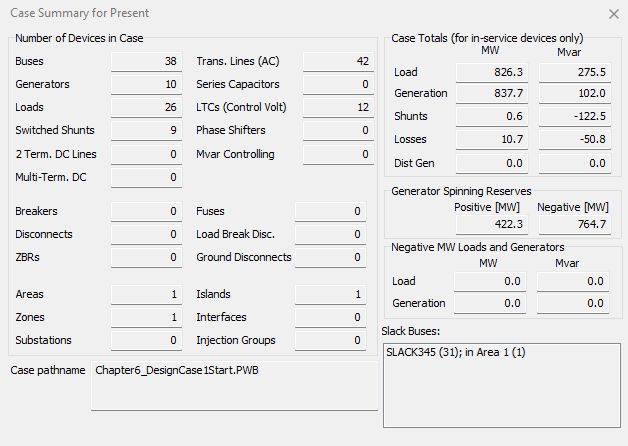
\includegraphics[width=1\linewidth]{figures/case_summary_existing}
	\caption{Case summary for existing system}
	\label{fig:casesummaryexisting}
\end{figure}
\subsection{Contingency Analysis}
PowerWorld's contingency analysis examines conditions when each element of the power system is taken offline. It reveals vulnerability in the 69 kV network in three contingency violations. Specifically, loss of either the PINE138 transformer or the PINE69-APPLE69 line results in overload, with the OAK69-BUCKEYE69 line experiencing loading up to 110.8\% of its thermal limit. These violations suggest that the existing infrastructure is approaching its capacity limits. 

These results are summarized in Table \ref{tab:violations}. A zoomed-in view of the affected areas of the power system is shown in Figure \ref{fig:baseviolations}.
\begin{table}[htbp]
	\caption{Line violations in contingency analysis}
	\begin{center}
		\begin{tabular}{|l|c|c|c|}
			\hline
			\textbf{Contingency} & \textbf{Flow(A)} & \textbf{Limit(A)} & \textbf{\%} \\
			\hline
			\textit{PINE138-PINE69 Xfmr:} & & & \\
			OAK69-BUCKEYE69 & 760.3 & 686.1 & 110.8 \\
			BUCKEYE69-APPLE69 & 454.2 & 418.4 & 108.6 \\
			\hline
			\textit{PINE69-APPLE69 Line:} & & & \\
			OAK69-BUCKEYE69 & 699.2 & 686.1 & 101.9 \\
			\hline
		\end{tabular}
		\label{tab:violations}
	\end{center}
\end{table}
\begin{figure}[tbph]
	\centering
	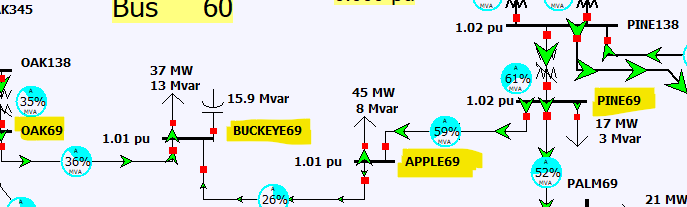
\includegraphics[width=1\linewidth]{figures/base_violations}
	\caption{Existing contingency violations - problem area}
	\label{fig:baseviolations}
\end{figure}
\section{Design Solutions}
\subsection{Design Options Considered}
\begin{itemize}
	\item Transmission line alternatives
	\item Voltage level considerations
	\item Transformer placement options
\end{itemize}

\subsection{Technical Analysis}
\begin{itemize}
	\item Power flow studies
	\item Contingency analysis results
	\item System performance improvements
\end{itemize}

\section{Economic Analysis}
\subsection{Cost Components}
\begin{itemize}
	\item Fixed costs (lines, transformers, substations)
	\item Variable costs (distance-based)
	\item Loss reduction benefits
\end{itemize}

\subsection{Solution Comparison}
\begin{table}[htbp]
	\caption{Cost Comparison of Design Options}
	\begin{center}
		\begin{tabular}{|c|c|c|c|}
			\hline
			\textbf{Design Option} & \textbf{Capital Cost} & \textbf{Loss Savings} & \textbf{Net Cost} \\
			\hline
			Option 1 & & & \\
			\hline
			Option 2 & & & \\
			\hline
		\end{tabular}
		\label{tab:costs}
	\end{center}
\end{table}

\section{Recommended Solution}
\begin{itemize}
	\item Final design selection
	\item Technical justification
	\item Economic justification
	\item Implementation considerations
\end{itemize}

\section{Conclusion}
Summary of key findings and recommendations
	
\begin{thebibliography}{00}
	\bibitem{b1} PowerWorld Corporation, "PowerWorld Simulator Manual," 2024.
	\bibitem{b2} IEEE Standard 1547-2018, "IEEE Standard for Interconnection and Interoperability of Distributed Energy Resources with Associated Electric Power Systems Interfaces."
\end{thebibliography}

\end{document}